\documentclass[pdftex,a4paper,10pt,twoside,titlepage]{article}
\usepackage[italian]{babel}
\usepackage[utf8]{inputenc}
\usepackage{fancyhdr,graphicx}
\usepackage[hmargin=2cm,vmargin=2cm,a4paper]{geometry}
\usepackage{hyperref}
\usepackage{xcolor}
\usepackage{multirow}
\pagestyle{fancy}
\lhead{\scshape Curriculum Vitae}
\rhead{\itshape Mauro Donadeo}
\rfoot{\footnotesize pag. \thepage}
\cfoot{}
\lfoot{{\footnotesize Update to: June 2013}}
\renewcommand{\headrulewidth}{.5pt}
\renewcommand{\footrulewidth}{.5pt}
%\renewcommand{\LettrineFontHook}{\color[gray]{0.5}}
%\renewcommand*\familydefault{\sfdefault}
\renewcommand*\labelitemi{$\textcolor{black!30}{\bullet}$}
%\definecolor{listings-comment-color}{RGB}{20,0,0}

\begin{document}
\begin{center}
\rule{.8 \textwidth}{1pt}\\[5pt]
\begin{minipage}{.55\textwidth}
	\LARGE\textbf{Mauro Donadeo}\\[16pt]
	\footnotesize Via Isonzo 136/7 \\ 
	35143 - Padova (PD)\\
	email: \texttt{mauro.donadeo@gmail.com}\\
	\footnotesize {Tel. +39 346 784 6243}\\
	\footnotesize Nationality: Italian\\
	\footnotesize {Skype: mauro.donadeo}\\
	\footnotesize{born on the 18th January 1986}\\
%	\footnotesize Stato civile: Celibe\\
\end{minipage}
\begin{minipage}{.25\textwidth}
	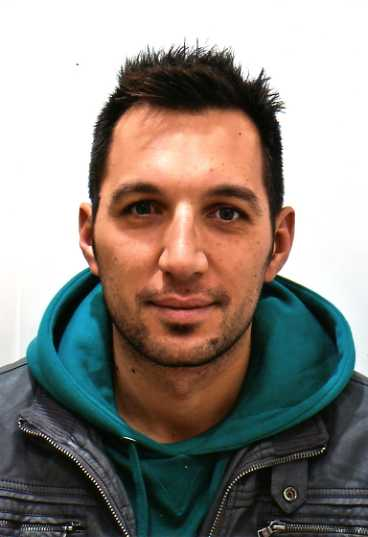
\includegraphics[width=\textwidth]{io.jpg}
\end{minipage}
\rule{.8 \textwidth}{1pt}\\[5pt]
\end{center}
%\vspace{0.5cm}
\section*{Work Experience}
\begin{tabular}[h]{l p{0.7\textwidth}}
\footnotesize{July 2012 - Today} & Research grant at University of Padua - DEI \\
 & Creation of a library for hand detection and hand gesture recognition, 
 through images acquired with low cost devices  (i.e. Microsoft Kinect). The acquisition system was
developed in \textit{C++} with the libraries \textit{OpenCV, OpenNI, VTK, PCL e Qt}.\\
 & \\
\footnotesize{Jan. 2012 - June. 2012} & Software engineer at University of Padua - DPG.\\
& Develop of a gesture recognition system with images acquired through MS Kinect. The system was
developed in C++ with the libraries \textit{OpenCV} and \textit{OpenNI}. The visual feedback was reproduced with \textit{Unity 3D}.
This project was developed within the CEEDs European Project (http//ceeds-project.eu).\\
&\\
\footnotesize{Nov. 2011 - Dec. 2011} & Web designer at SimNumerica srl.\\
& Creation web page with Drupal CMS. Focus on: integration and adaptation of login-module, news-slider, 
		ticketing module and creating a wiki for administrator users. \\
&\\
\footnotesize{Sept. 2008 - Aug. 2009} &  Computer assistant for the Certification Courses Office - SID (University of Padua)\\
& Comparison between didactic database of the University and the Ministerial data.
 Development of a web application to automate the validation of students classes and study plans. The new system allowed
 to speed-up generations of diplomas and delivery time by 50\%.\\
&\\
\footnotesize{Dec. 2007  -  Aug. 2008} & Computer assistant in the office Technical and Network coordination at the Regione Veneto.\\
 & Design and implementation of the portal {\texttt overnetwork.it} based on \textit{Joomla CMS}
  with focus on: creation of system of ticketing (with mail alert system) and new system of users profiling. Participation in 802.1x project.\\
&\\
\footnotesize{Sept. 2005 - Oct. 2007} & Postman in the province of Padua.
\end{tabular} 
\section*{Education}
\begin{itemize}
	\item Master's Degree in Computer Engineering (University of Padua, October 2011).\\
	Thesis: {\itshape 3D Real time video conferencing system based on Microsoft Kinect sensor: design and implementation } (grade 92/110)
	\item Bachelor's Degree in Computer Engineering (University of Padua, April 2008). \\Thesis:
	{\itshape Java Simulator for the Lego NXT robotic system: design and implementation} (grade 90/110)
	\item High School Diploma, Computer Science  (I.T.I.S. A. Meucci of Casarano (LE), 2004) (grade 85/100)
\end{itemize}

\section*{Computer skills}
\begin{itemize}
	\item \textbf{S.O.:} Gnu/Linux: from installation to configuration and various operating system; various other Microsoft operating system.
	\item \textbf{Programming:} 
	\begin{itemize}
	\item C/C++/C\#(beginner);
	\item Java
	\item Php MySql.
	\end{itemize}
	\item \textbf{Other:}
	\begin{itemize}
	\item library for the computer vision: Directx10, OpenNI, OpenGL(beginner), OpenCV, Qt4;
	\item developing system of stereo acquisition and MS Kinect;
	\item IDE: NetBeans, Visual Studio 2010, QtCreator;
	\item Unity 3D Game Engine, PCL(beginner);
	\item vim, Matlab, Office, NXC, \LaTeX, Git, svn.
	\end{itemize}
\end{itemize}
\section*{Language skills}
\begin{itemize}
	\item \textbf{Italian:} native;
	\item \textbf{English:} intermediate;
	\item \textbf{Spanish:} advanced.
\end{itemize}
\section*{Personal Interests}
\begin{itemize}
	\item Images video  editing, computer science, mobile technology
	\item Hobbies: swimming, jogging, football, reading, travelling
\end{itemize}
\vfill
%I authorise the use of my personal data according to Legislative Decree No. 196/03.
\vspace{1cm}
\end{document}
